%%%%%%%%%%%%%%%%%%%%%%%%%%%%%%%%%%%%%%%%%%%%%%%%%%%%%%%%%%%%%%%%%%%%%%%%%%%%%%
%
% Section file included in main project file using \input{}
%
% Assumes that LaTeX2e macros and packages defined in cg_comp.sty are
%   available
%
%%%%%%%%%%%%%%%%%%%%%%%%%%%%%%%%%%%%%%%%%%%%%%%%%%%%%%%%%%%%%%%%%%%%%%%%%%%%%%

 \section{Classical Guitar Compensation\label{sct:comp}}


\red{Strategy: Use $\Delta S$ to compensate for bending stiffness, and $\Delta N$ to compensate for tension increases arising from fretting. Doing so predicts that $\Delta S \approx 3$~mm for the Alhambra 8P with light-tension strings, or about twice the saddle setback that is actually manufactured.}


\begin{table}%[htbp]
  \centering
  \caption{\label{tbl:ej43_setbacks} Predicted setbacks for the D'Addario Pro-Arte Nylon Classical Guitar Strings -- Light Tension (EJ43) on the Alhambra 8P classical guitar.}
    \begin{tabular}{lcccc}
    \hline \hline
    String  & $\Delta S$~(mm) & $\Delta N$~(mm) \\
    \hline
    J4301 & 1.91 & -0.31 \\
    J4302 & 1.37 & -0.12 \\
    J4303 & 4.38 & -0.79 \\
    J4304 & 1.92 & -0.30 \\
    J4305 & 2.29 & -0.31 \\
    J4306 & 2.08 & -0.16 \\
    \hline \hline
    Mean & 2.32 & -0.33 \\
    \hline
    \end{tabular}%
  \label{tab:addlabel}%
\end{table}%


 \begin{figure}
  \centering
  \begin{subfigure}[b]{0.45\textwidth}
   \centering
   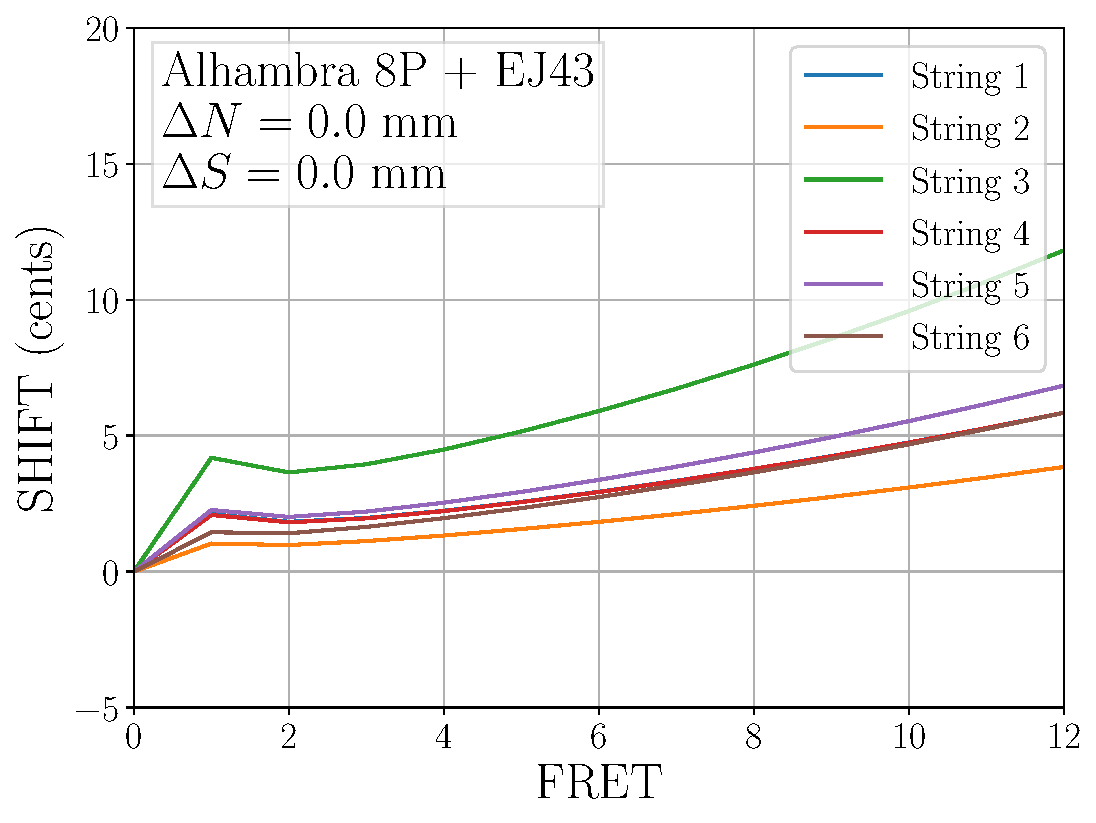
\includegraphics[width=3.25in]{figures/shift_alhambra8p_ej43_null}
   \caption{Uncompensated}
   \label{fig:shift_alhambra8p_ej43_null}
  \end{subfigure}
  \hspace{0.25in}
  \begin{subfigure}[b]{0.45\textwidth}
   \centering
   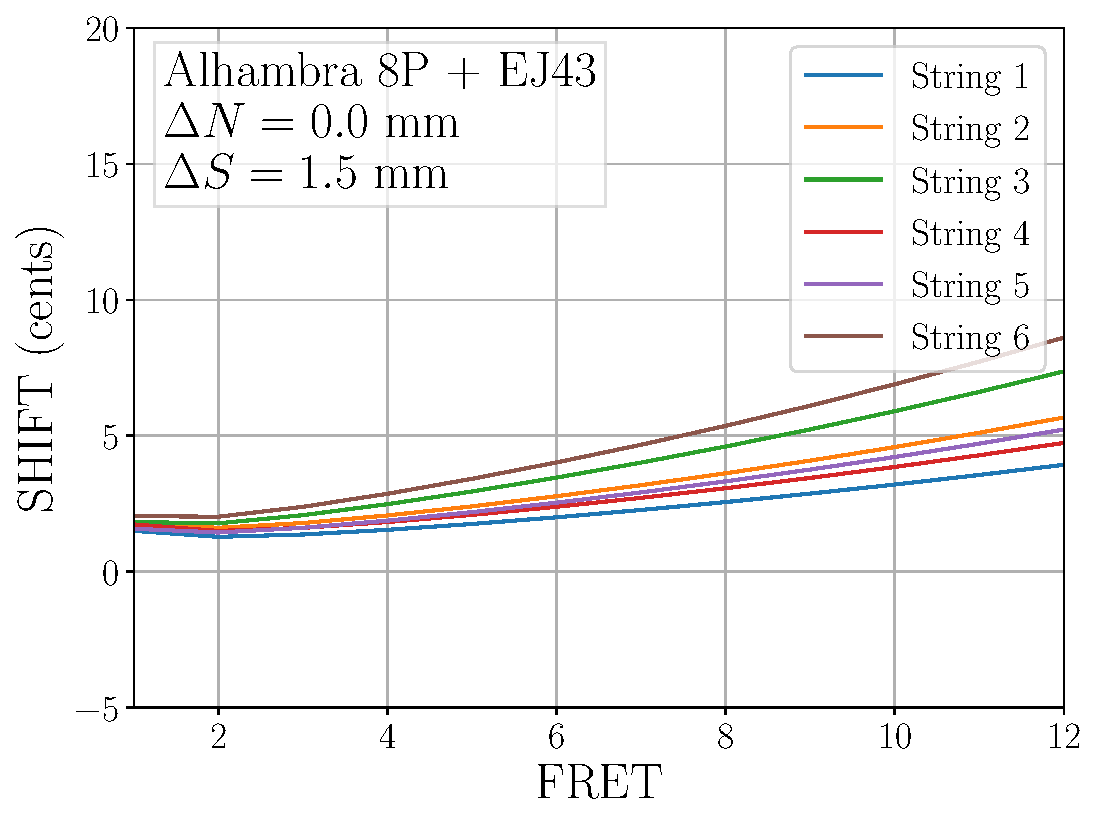
\includegraphics[width=3.25in]{figures/shift_alhambra8p_ej43_factory}
   \caption{Factory guitar}
   \label{fig:shift_alhambra8p_ej43_factory}
  \end{subfigure}
  \par\vspace{0.25in}
  \begin{subfigure}[b]{0.45\textwidth}
   \centering
   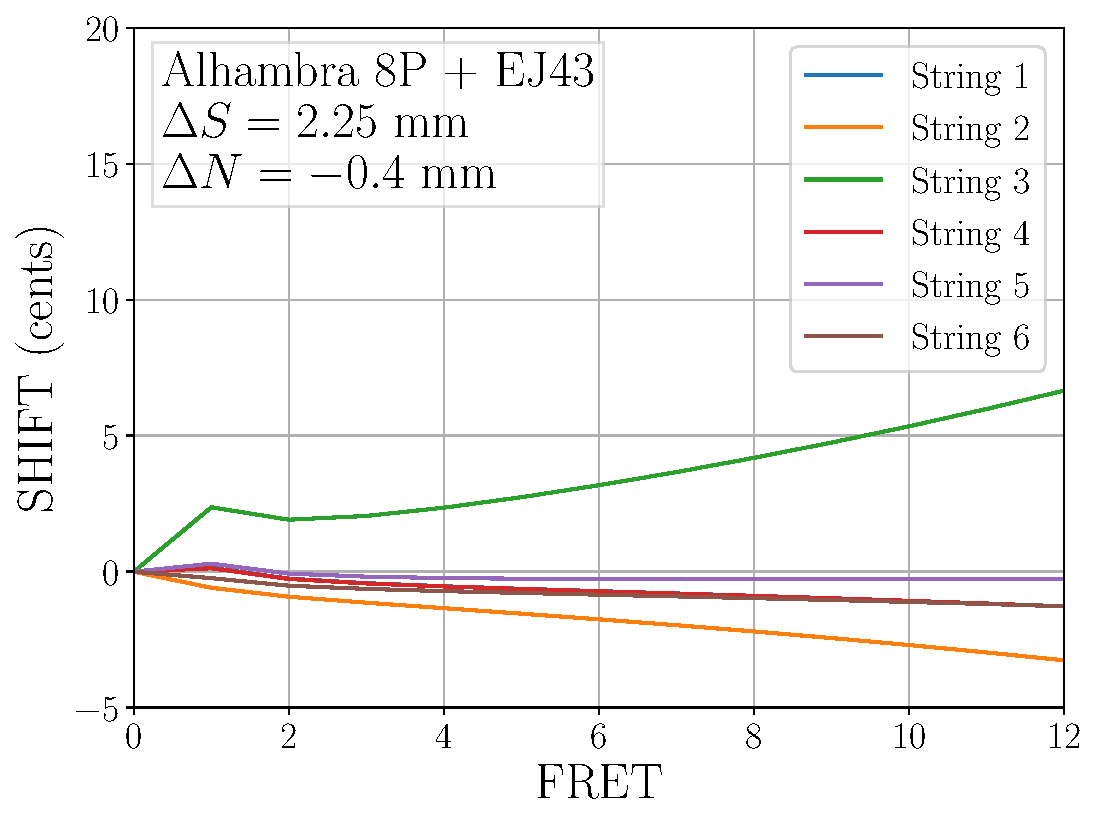
\includegraphics[width=3.25in]{figures/shift_alhambra8p_ej43_mean}
   \caption{Mean compensation}
   \label{fig:shift_alhambra8p_ej43_mean}
  \end{subfigure}
  \hspace{0.25in}
  \begin{subfigure}[b]{0.45\textwidth}
   \centering
   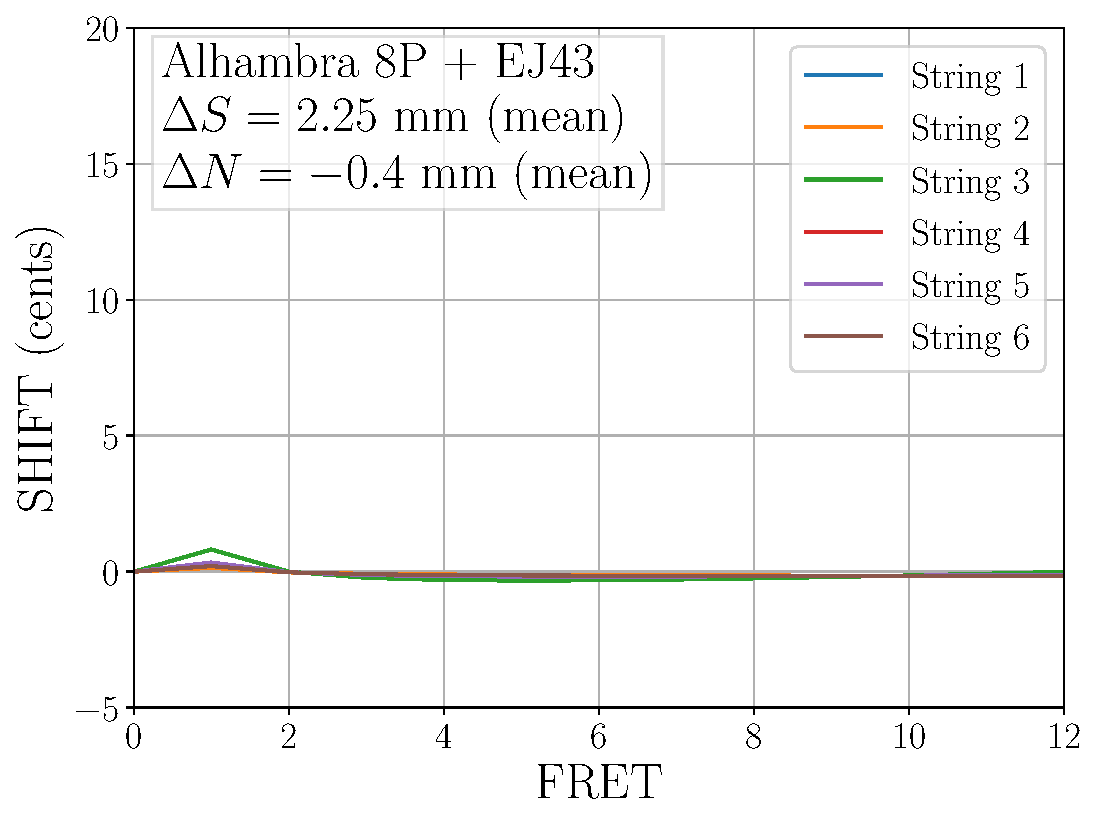
\includegraphics[width=3.25in]{figures/shift_alhambra8p_ej43_full}
   \caption{Full compensation}
   \label{fig:shift_alhambra8p_ej43_full}
  \end{subfigure}
  \caption{\label{fig:compensation} Frequency shift (in cents) for an Alhambra 8P guitar with D'Addario Pro-Arte Nylon Classical Guitar Strings -- Light Tension (EJ43). Four different strategies of saddle and nut compensation are illustrated.}
 \end{figure}


\begin{table}%[htbp]
  \centering
  \caption{\label{tbl:ej46_setbacks} Predicted setbacks for the D'Addario Pro-Arte Nylon Classical Guitar Strings -- Hard Tension (EJ46) on the Alhambra 8P classical guitar.}
    \begin{tabular}{lcccc}
    \hline \hline
    String  & $\Delta S$~(mm) & $\Delta N$~(mm) \\
    \hline
    J4601 & 3.91 & -1.20 \\
    J4602 & 2.84 & -0.49 \\
    J4603 & 3.00 & -0.34 \\
    J4604 & 2.77 & -0.55 \\
    J4605 & 2.03 & -0.20 \\
    J4606 & 3.04 & -0.31 \\
    \hline \hline
    Mean & 2.93 & -0.52 \\
    \hline
    \end{tabular}%
  \label{tab:addlabel}%
\end{table}%


 \begin{figure}
  \centering
  \begin{subfigure}[b]{0.45\textwidth}
   \centering
   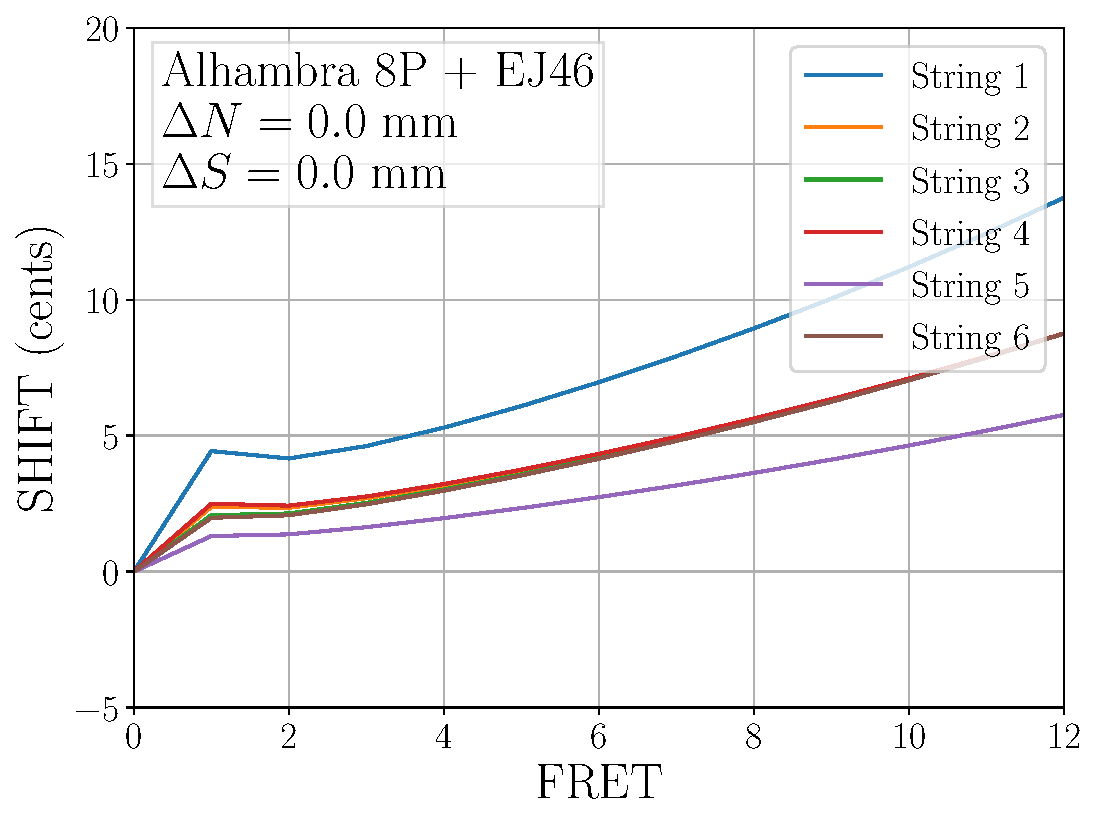
\includegraphics[width=3.25in]{figures/shift_alhambra8p_ej46_null}
   \caption{Uncompensated}
   \label{fig:shift_alhambra8p_ej46_null}
  \end{subfigure}
  \hspace{0.25in}
  \begin{subfigure}[b]{0.45\textwidth}
   \centering
   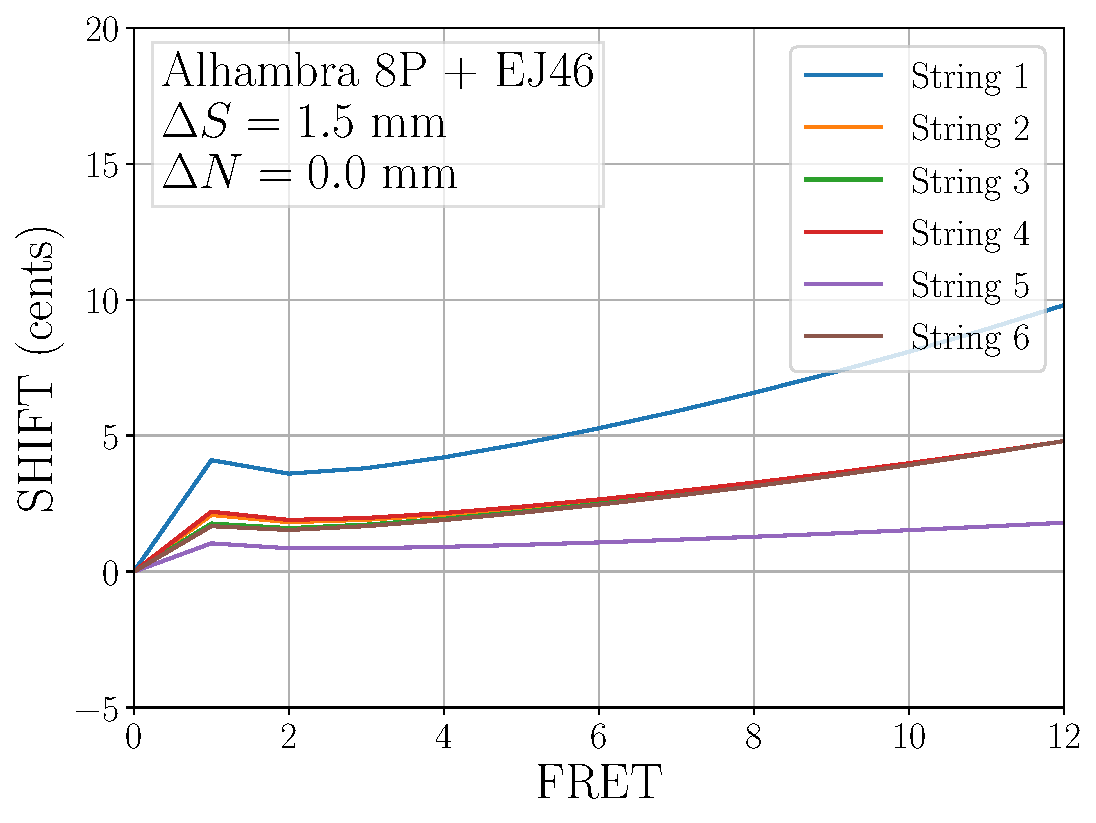
\includegraphics[width=3.25in]{figures/shift_alhambra8p_ej46_factory}
   \caption{Factory guitar}
   \label{fig:shift_alhambra8p_ej46_factory}
  \end{subfigure}
  \par\vspace{0.25in}
  \begin{subfigure}[b]{0.45\textwidth}
   \centering
   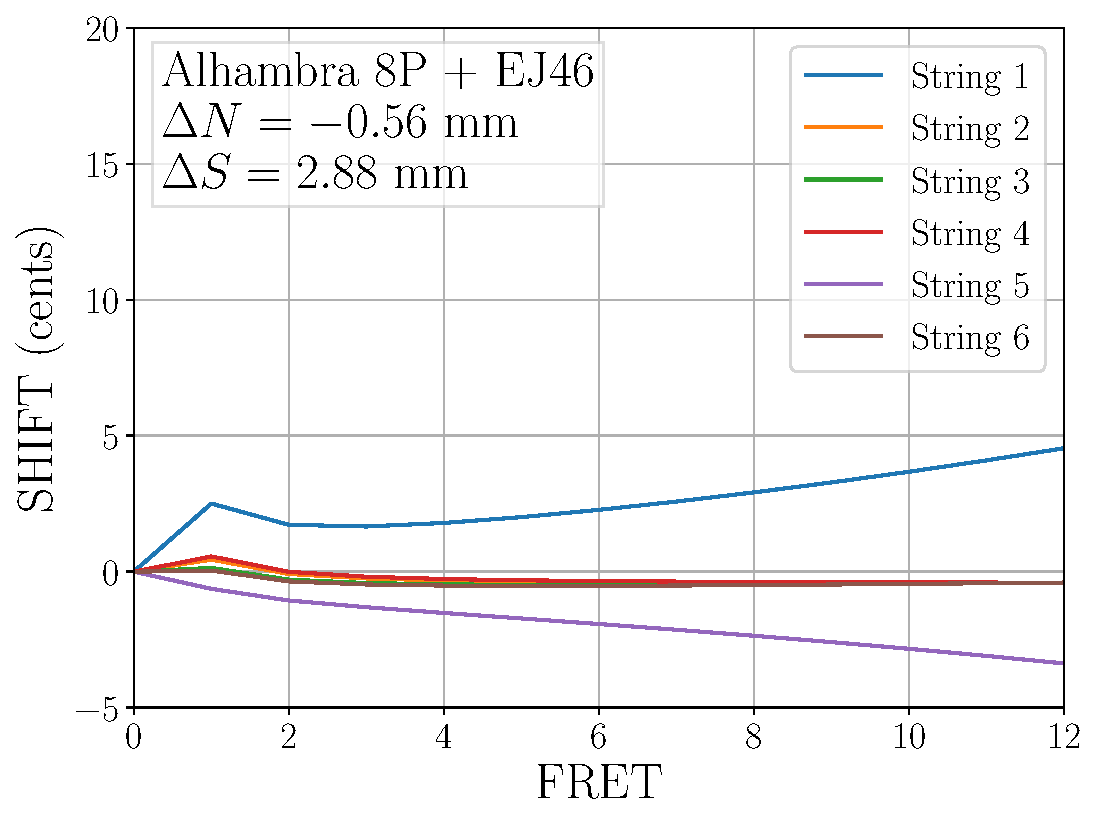
\includegraphics[width=3.25in]{figures/shift_alhambra8p_ej46_mean}
   \caption{Mean compensation}
   \label{fig:shift_alhambra8p_ej46_mean}
  \end{subfigure}
  \hspace{0.25in}
  \begin{subfigure}[b]{0.45\textwidth}
   \centering
   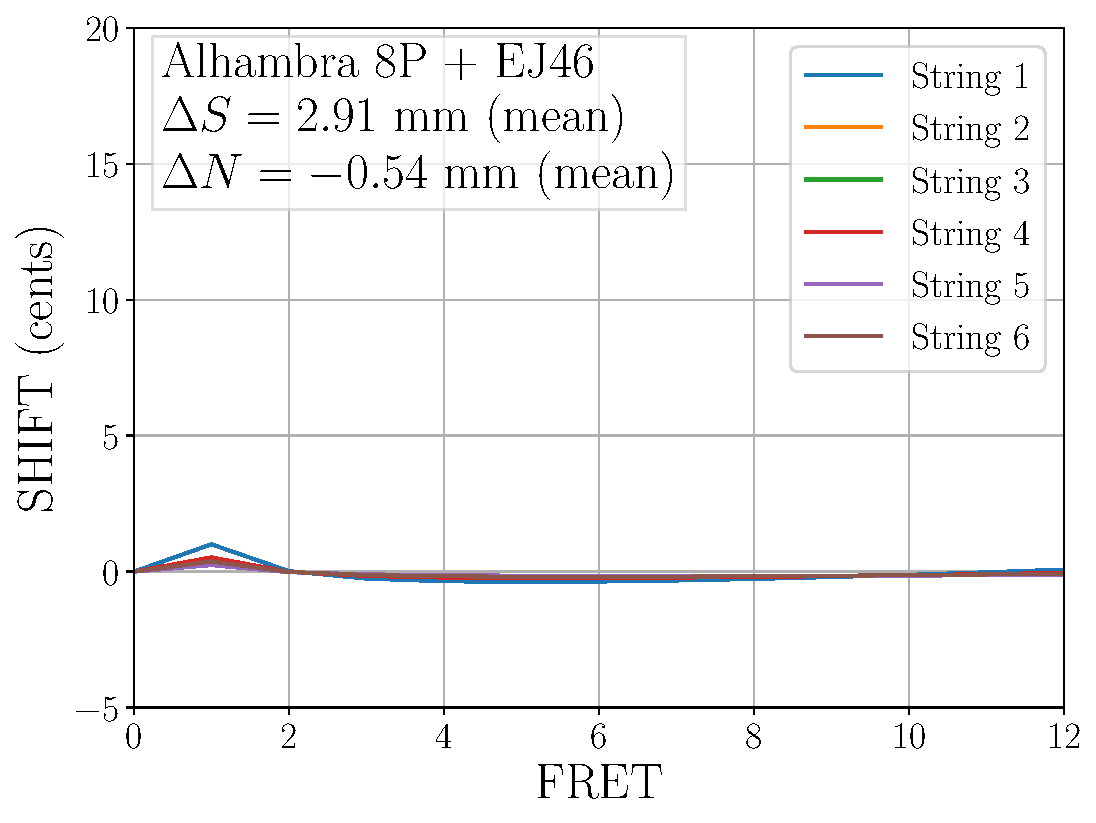
\includegraphics[width=3.25in]{figures/shift_alhambra8p_ej46_full}
   \caption{Full compensation}
   \label{fig:shift_alhambra8p_ej46_full}
  \end{subfigure}
  \caption{\label{fig:compensation} Frequency shift (in cents) for an Alhambra 8P guitar with D'Addario Pro-Arte Nylon Classical Guitar Strings -- Hard Tension (EJ46). Four different strategies of saddle and nut compensation are illustrated.}
 \end{figure}

\begin{table}%[htbp]
  \centering
  \caption{\label{tbl:ej44_setbacks} Predicted setbacks for the D'Addario Pro-Arte Nylon Classical Guitar Strings -- Extra Hard Tension (EJ44) on the Alhambra 8P classical guitar.}
    \begin{tabular}{lcccc}
    \hline \hline
    String  & $\Delta S$~(mm) & $\Delta N$~(mm) \\
    \hline
    J4401 & 1.93 & -0.29 \\
    J4402 & 3.39 & -0.67 \\
    J4403 & 4.44 & -0.73 \\
    J4404 & 2.77 & -0.55 \\
    J4405 & 2.03 & -0.20 \\
    J4406 & 3.05 & -0.30 \\
    \hline \hline
    Mean & 2.94 & -0.46 \\
    \hline
    \end{tabular}%
  \label{tab:addlabel}%
\end{table}%


 \begin{figure}
  \centering
  \begin{subfigure}[b]{0.45\textwidth}
   \centering
   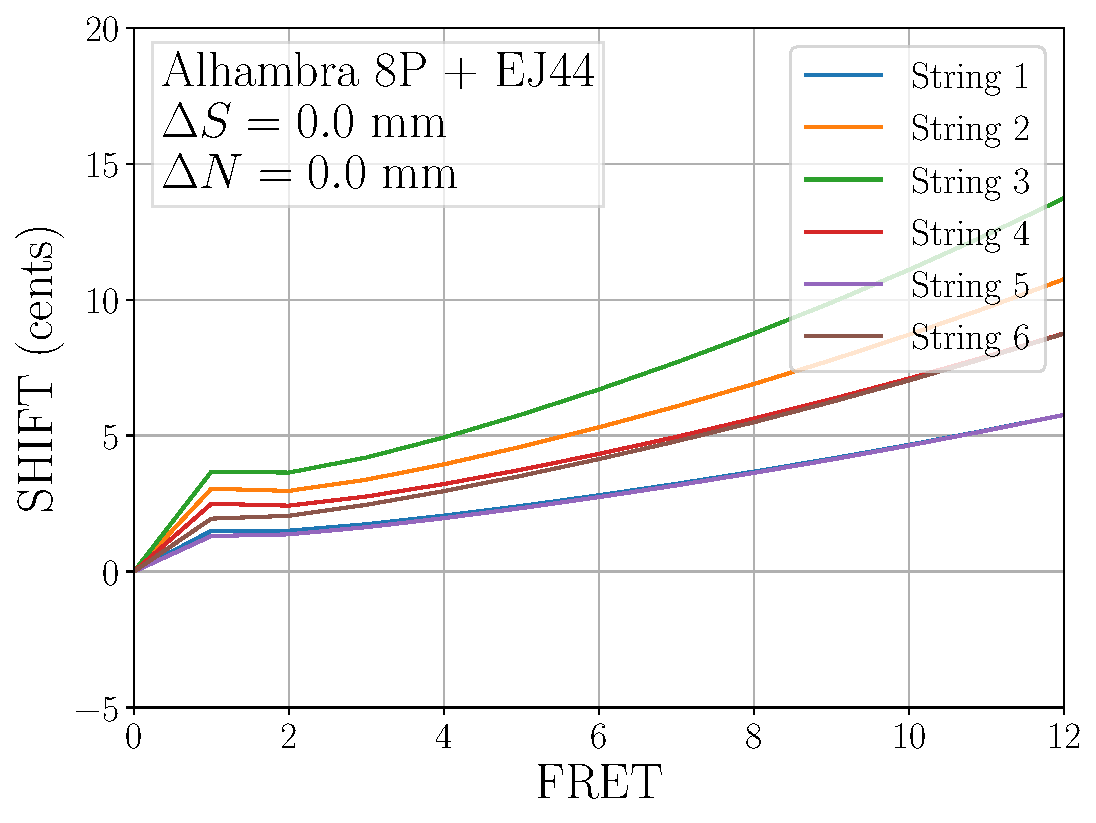
\includegraphics[width=3.25in]{figures/shift_alhambra8p_ej44_null}
   \caption{Uncompensated}
   \label{fig:shift_alhambra8p_ej44_null}
  \end{subfigure}
  \hspace{0.25in}
  \begin{subfigure}[b]{0.45\textwidth}
   \centering
   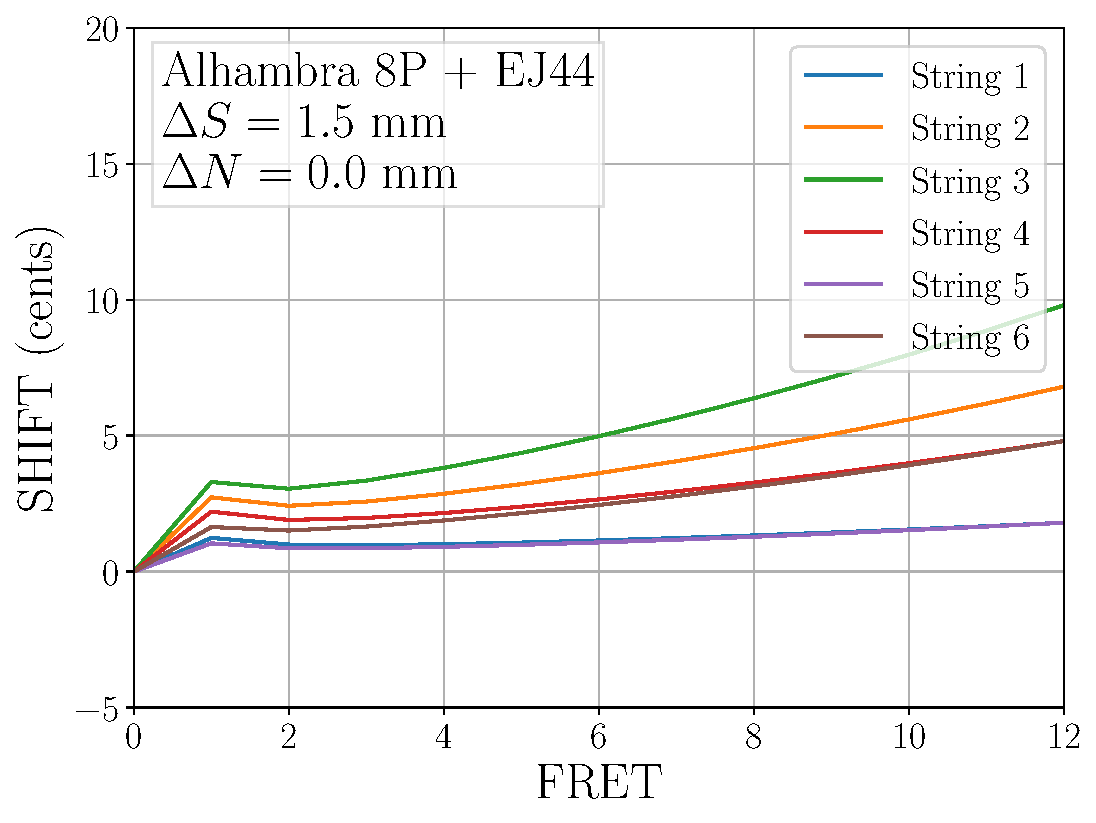
\includegraphics[width=3.25in]{figures/shift_alhambra8p_ej44_factory}
   \caption{Factory guitar}
   \label{fig:shift_alhambra8p_ej44_factory}
  \end{subfigure}
  \par\vspace{0.25in}
  \begin{subfigure}[b]{0.45\textwidth}
   \centering
   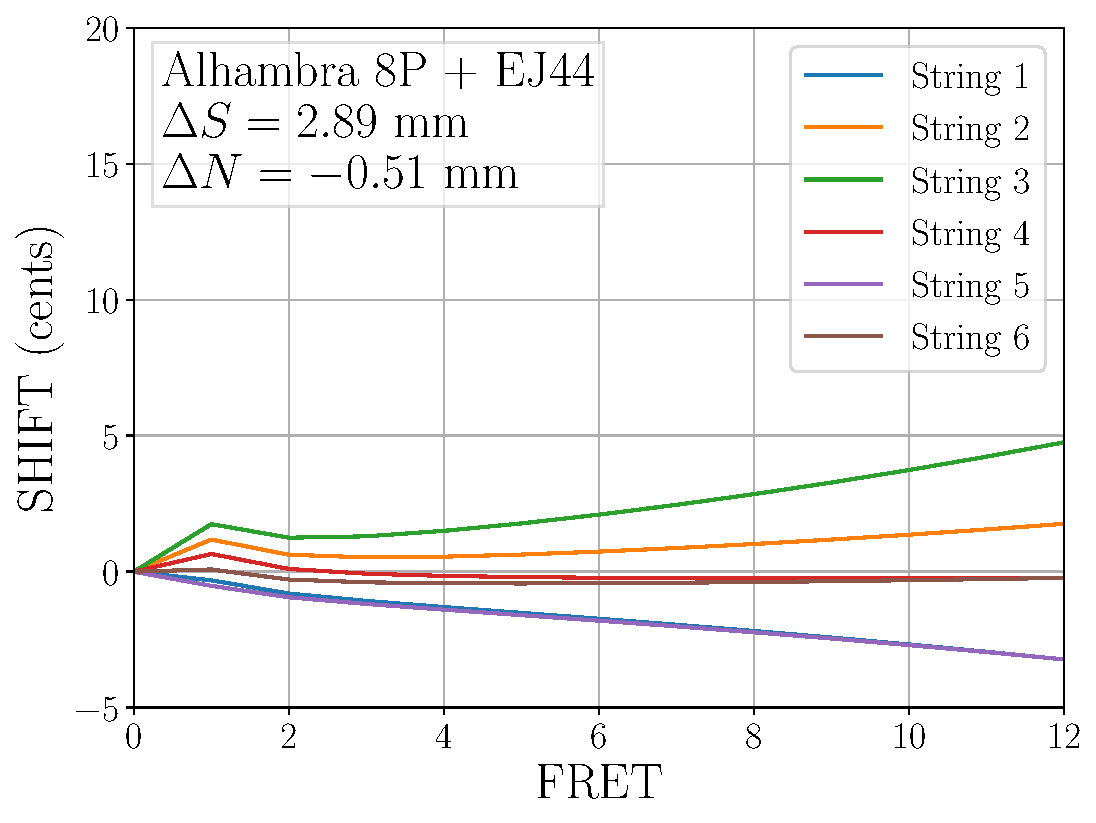
\includegraphics[width=3.25in]{figures/shift_alhambra8p_ej44_mean}
   \caption{Mean compensation}
   \label{fig:shift_alhambra8p_ej44_mean}
  \end{subfigure}
  \hspace{0.25in}
  \begin{subfigure}[b]{0.45\textwidth}
   \centering
   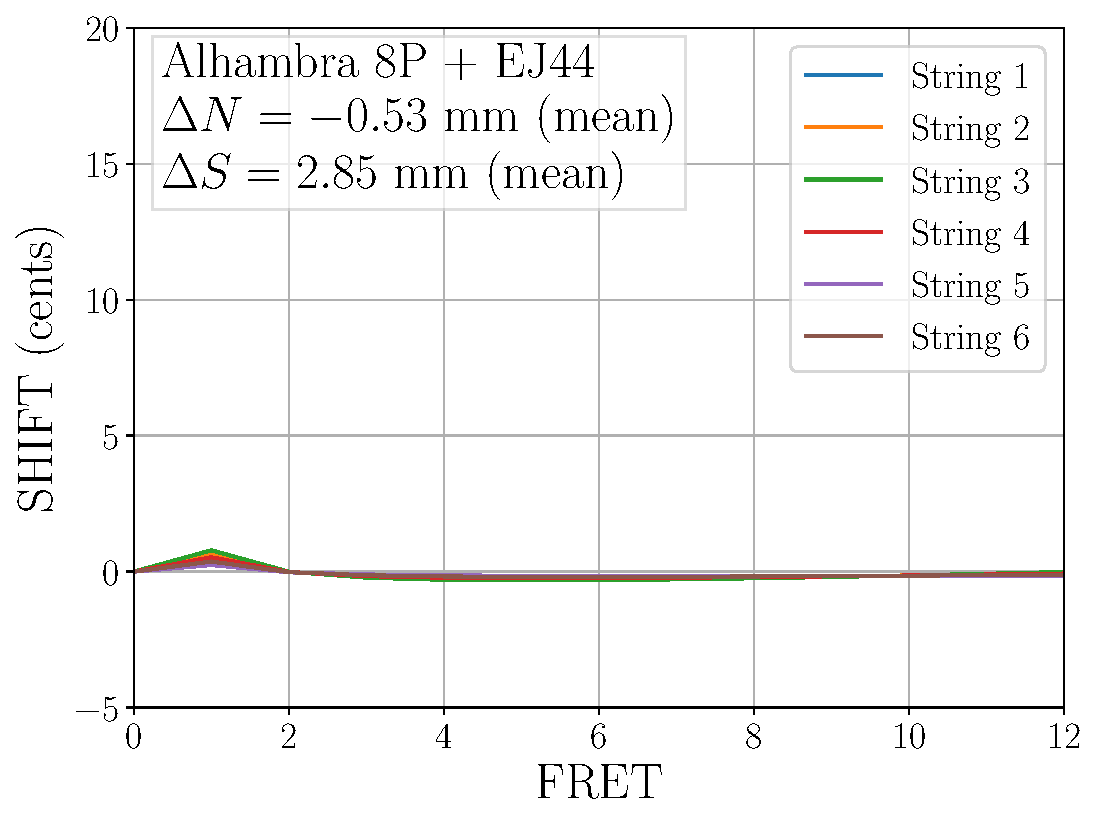
\includegraphics[width=3.25in]{figures/shift_alhambra8p_ej44_full}
   \caption{Full compensation}
   \label{fig:shift_alhambra8p_ej44_full}
  \end{subfigure}
  \caption{\label{fig:compensation} Frequency shift (in cents) for an Alhambra 8P guitar with D'Addario Pro-Arte Nylon Classical Guitar Strings -- Extra Hard Tension (EJ44). Four different strategies of saddle and nut compensation are illustrated.}
 \end{figure}


